\documentclass{tufte-handout}\usepackage[]{graphicx}\usepackage[]{color}
%% maxwidth is the original width if it is less than linewidth
%% otherwise use linewidth (to make sure the graphics do not exceed the margin)
\makeatletter
\def\maxwidth{ %
  \ifdim\Gin@nat@width>\linewidth
    \linewidth
  \else
    \Gin@nat@width
  \fi
}
\makeatother

\definecolor{fgcolor}{rgb}{0.345, 0.345, 0.345}
\newcommand{\hlnum}[1]{\textcolor[rgb]{0.686,0.059,0.569}{#1}}%
\newcommand{\hlstr}[1]{\textcolor[rgb]{0.192,0.494,0.8}{#1}}%
\newcommand{\hlcom}[1]{\textcolor[rgb]{0.678,0.584,0.686}{\textit{#1}}}%
\newcommand{\hlopt}[1]{\textcolor[rgb]{0,0,0}{#1}}%
\newcommand{\hlstd}[1]{\textcolor[rgb]{0.345,0.345,0.345}{#1}}%
\newcommand{\hlkwa}[1]{\textcolor[rgb]{0.161,0.373,0.58}{\textbf{#1}}}%
\newcommand{\hlkwb}[1]{\textcolor[rgb]{0.69,0.353,0.396}{#1}}%
\newcommand{\hlkwc}[1]{\textcolor[rgb]{0.333,0.667,0.333}{#1}}%
\newcommand{\hlkwd}[1]{\textcolor[rgb]{0.737,0.353,0.396}{\textbf{#1}}}%

\usepackage{framed}
\makeatletter
\newenvironment{kframe}{%
 \def\at@end@of@kframe{}%
 \ifinner\ifhmode%
  \def\at@end@of@kframe{\end{minipage}}%
  \begin{minipage}{\columnwidth}%
 \fi\fi%
 \def\FrameCommand##1{\hskip\@totalleftmargin \hskip-\fboxsep
 \colorbox{shadecolor}{##1}\hskip-\fboxsep
     % There is no \\@totalrightmargin, so:
     \hskip-\linewidth \hskip-\@totalleftmargin \hskip\columnwidth}%
 \MakeFramed {\advance\hsize-\width
   \@totalleftmargin\z@ \linewidth\hsize
   \@setminipage}}%
 {\par\unskip\endMakeFramed%
 \at@end@of@kframe}
\makeatother

\definecolor{shadecolor}{rgb}{.97, .97, .97}
\definecolor{messagecolor}{rgb}{0, 0, 0}
\definecolor{warningcolor}{rgb}{1, 0, 1}
\definecolor{errorcolor}{rgb}{1, 0, 0}
\newenvironment{knitrout}{}{} % an empty environment to be redefined in TeX

\usepackage{alltt}

%\documentclass{article}
\usepackage{graphicx}
%\setkeys{Gin}{width=\linewidth,totalheight=\textheight,keepaspectratio}
% Prints a trailing space in a smart way.
\usepackage{xspace}
\usepackage{hyperref}
\usepackage{amsmath}
\newcommand{\tthdump}[1]{#1}
\usepackage{makeidx}
\usepackage{tabularx}

%\makeindex

\begin{knitrout}
\definecolor{shadecolor}{rgb}{0.969, 0.969, 0.969}\color{fgcolor}\begin{kframe}


{\ttfamily\noindent\color{warningcolor}{\#\# Warning: No security definition has been found for the request}}\begin{verbatim}
## failed to load HTTP resource
\end{verbatim}


{\ttfamily\noindent\bfseries\color{errorcolor}{\#\# Error: 1: failed to load HTTP resource}}\end{kframe}
\end{knitrout}


\title{Buy On Gap trading report - S\&P 500}

\date{ 19 Dec 2013 }

\IfFileExists{upquote.sty}{\usepackage{upquote}}{}


\begin{document}
\maketitle

%\SweaveOpts{concordance=TRUE}
%\setkeys{Gin}{width=1.1\marginparwidth} %% Sweave

\section{Trade execution}
\subsection{Order executed}

% latex table generated in R 3.0.2 by xtable 1.7-1 package
% Fri Dec 20 05:10:31 2013
\begin{table}[ht]
\centering
\begin{tabular}{llrrrrrrr|r}
  \hline
 & Symbol & B.AvgPrc & B.Qty & S.AvgPrc & S.Qty & Profit & Comm. & Return \% & Closing Price \\ 
  \hline
1 & DRI & 51.39 & 1758 & 51.08 & 1758 & -549.86 & 19.14 & -0.61 & 50.96 \\ 
   \hline
\end{tabular}
\end{table}



\subsection{Stock Portfolio}
% latex table generated in R 3.0.2 by xtable 1.7-1 package
% Fri Dec 20 05:10:31 2013
\begin{table}[ht]
\centering
\begin{tabular}{llrrr}
  \hline
 & Symbol & Quantity & Closing price & Market price \\ 
  \hline
1 & ***NO-ASSET*** &  &  &  \\ 
   \hline
\end{tabular}
\end{table}



\section{Trading Matrix}


% latex table generated in R 3.0.2 by xtable 1.7-1 package
% Fri Dec 20 05:10:31 2013
\begin{table}[ht]
\begin{tabular}{lr}
   \hline
Portofolio Amount: & 89754.68 \\ 
  Asset Amount: & 0.00 \\ 
  Bought Amount: & 90335.52 \\ 
  Sold   Amount: & 89804.80 \\ 
  Commission   : & 19.14 \\ 
  P/L incl Comm: & -549.86 \\ 
  Ret incl Comm \%: & -0.61 \\ 
  S\&P 500 Ret \%: & -0.06 \\ 
   \hline
\end{tabular}
\caption{The commissions and daily returns are calculated based on the closed position.
The open position is present in the portofolio and assume closing on the next open market.
Portofolio amount is the open order with today closing price.} 
\end{table}



% \section{Trade Slippage}
% 
% <<slippage, echo = FALSE , results='asis'>>=
% 
% colnames(slippage) <- c('Symbol','Open Slippage %', 'Close Slippage %');
% print(xtable(slippage),floating=FALSE,);
% @


\title{Buy On Gap trading report - S\&P 600}
\maketitle

\section{Trade execution}
\subsection{Order executed}


% latex table generated in R 3.0.2 by xtable 1.7-1 package
% Fri Dec 20 05:10:31 2013
\begin{table}[ht]
\centering
\begin{tabular}{llrrrrrrr|r}
  \hline
 & Symbol & B.AvgPrc & B.Qty & S.AvgPrc & S.Qty & Profit & Comm. & Return \% & Closing Price \\ 
  \hline
1 & MCS & 13.35 & 1535 & 13.21 & 1535 & -230.60 & 15.70 & -1.12 & 13.23 \\ 
  2 & NEOG & 45.33 & 455 & 43.88 & 455 & -663.10 & 4.90 & -3.21 & 43.92 \\ 
   \hline
\end{tabular}
\end{table}



\subsection{Stock Portfolio}
% latex table generated in R 3.0.2 by xtable 1.7-1 package
% Fri Dec 20 05:10:31 2013
\begin{table}[ht]
\centering
\begin{tabular}{llrrr}
  \hline
 & Symbol & Quantity & Closing price & Market price \\ 
  \hline
1 & CENTA & 2718 & 6.42 & 17449.56 \\ 
   \hline
\end{tabular}
\end{table}



\section{Trading Matrix}

% latex table generated in R 3.0.2 by xtable 1.7-1 package
% Fri Dec 20 05:10:32 2013
\begin{table}[ht]
\begin{tabular}{lr}
   \hline
Portofolio Amount: & 97953.73 \\ 
  Asset Amount: & 17449.56 \\ 
  Bought Amount: & 41116.85 \\ 
  Sold   Amount: & 40243.75 \\ 
  Commission   : & 20.60 \\ 
  P/L incl Comm: & -893.70 \\ 
  Ret incl Comm \%: & -1.71 \\ 
  S\&P 600 Ret \%: & -0.87 \\ 
   \hline
\end{tabular}
\caption{The commissions and daily returns are calculated based on the closed position.
The open position is present in the portofolio and assume closing on the next open market.
Portofolio amount is the open order with today closing price.} 
\end{table}



% \section{Trade Slippage}
% 
% <<slippage_sp600, echo = FALSE , results='asis'>>=
% 
% colnames(slippage) <- c('Symbol','Open Slippage %', 'Close Slippage %');
% print(xtable(slippage),floating=FALSE,);
% @

\newpage
\section{News}

%\begin{margintable}

% latex table generated in R 3.0.2 by xtable 1.7-1 package
% Fri Dec 20 05:10:32 2013
\begin{tabularx}{\textwidth}{rX}
  \hline
 & DRI \\ 
  \hline
1 &  Darden Restaurants Inc. (DRI) includes some of the most well known restaurant chains in the country including Red Lobster, Olive Garden and LongHorn SteakHouse.  \\ 
  2 &  Darden Restaurants Inc. ( DRI ) is due to issue its quarterly earnings report in the upcoming extended-hours session. Given its history, traders can expect light trading in the issue immediately following its quarterly earnings announcement.  \\ 
  3 &  Darden currently expects diluted net earnings per share for fiscal year 2014 to decline between 15\% and 20\% compared to fiscal 2013.  \\ 
  4 &  (Reuters) - Darden Restaurants Inc said it would sell or spin off its Red Lobster business, buckling under pressure from activist investor Barington Capital Group.  \\ 
  5 &  Darden Restaurants Inc. plans to separate its struggling Red Lobster business from the rest of the casual-dining company, while also saying it intends to suspend acquisitions.  \\ 
  6 &  Darden Restaurants Inc. is looking to either spin off or sell Red Lobster, part of its plan to boost shareholder value. The company, which also runs Olive Garden and other restaurants, said Thursday that it is also suspending the opening of new Olive ...  \\ 
  7 &  (Reuters) - Darden Restaurants Inc ($>$$>$ Darden Restaurants, Inc.), under pressure from activist investor Barington Capital Group because of sliding profits, said it would sell or spin off its struggling Red Lobster chain.  \\ 
  8 &  Darden Restaurants, Inc. (NYSE:DRI) plans to unload Red Lobster, following months of pressure to break up from Barington Capital Group, an activist hedge fund.  \\ 
  9 &  Alimera Sciences Inc. (ALIM, \$4.26, +\$1.71, +67.06\%) and pSivida Corp. (PSDV, \$4.18, +\$1.21, +40.74\%)(PVA.AU) shares soared after Alimera disclosed they were in talks with the U.S.  \\ 
  10 &  Let's have a look on Few Hot Stocks:Darden Restaurants, Inc. (NYSE:DRI), ConAgra Foods, Inc. (NYSE:CAG), Alimera Sciences Inc (NASDAQ:ALIM), AK Steel Holding Corporation (NYSE:AKS) Darden Restaurants, Inc. (NYSE:DRI) was trading lower by -2.53 ...  \\ 
   \hline
\end{tabularx}


%\end{margintable}

\newpage
\section{Individual contract}
\begin{fullwidth}
\begin{knitrout}
\definecolor{shadecolor}{rgb}{0.969, 0.969, 0.969}\color{fgcolor}\begin{kframe}


{\ttfamily\noindent\bfseries\color{errorcolor}{\#\# Error: chartSeries requires an xtsible object}}\end{kframe}
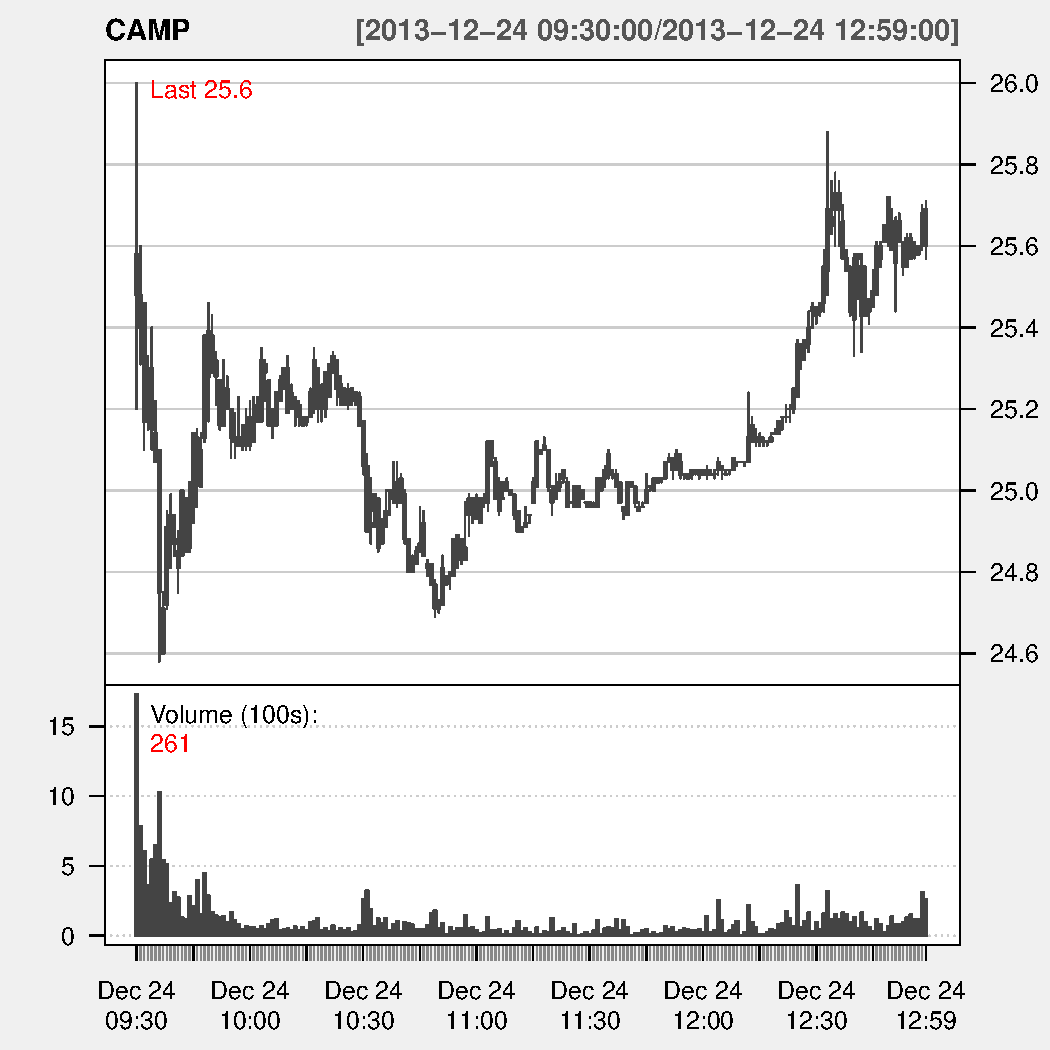
\includegraphics[width=\maxwidth]{/home/jhleong/dev/R/buy_on_gap/BuyOnGap_report/figure/price_chart} 

\end{knitrout}


\end{fullwidth}
\end{document}
